\documentclass{article}
\usepackage[utf8]{inputenc}
\usepackage[T1]{fontenc}
\usepackage{scrextend}
\usepackage{gensymb}
\usepackage{graphicx}
\usepackage[numbers]{natbib}
\usepackage{hyperref} 
\graphicspath{ {./img/procedure/}{./img/results/}{./img/intro/}{./img/task/}}
\title{Spatial problem solving and collaboration in virtual reality}
\author{Marcel Bechtold}
\date{\today}


\begin{document}

\maketitle


\section{Abstract}

Lorem ipsum

\section{Introduction} \label{sec:introduction}
\paragraph{What is problem solving}
Problem solving is a meanwhile well established field in cognitive psychology. The literature suggests that different sub processes of problem solving need to be considered in order to understand the whole process. The relevant sub-processes are the perception of the task, understanding the problem, activating foreknowledge, manipulating the given information, dividing the problem into subgoals, developing a plan, detecting errors and finding and validating results. The sub-processes of problem solving can also be investigated separately. Problem solving in general can be defined by the attempt to transition from a given initial state to a goal state. Furthermore it is necessary that there must be some kind of barrier that prevents one from achieving the goal state directly. \cite{muesseler2015allgemeine}

\paragraph{Methods in problem solving research}
In previous research some common methods of investigating problem solving have been established. The main goal it to identify the cognitive and neuronal processes of problem solving. A popular method is eye tracking because it allows to identify which informations of a problem are being looked at. \cite{underwood2005}  Furthermore neuropsychological studies are used to investigate which brain areas are responsible for certain aspects of problem solving. \cite{Karnath2006} In general there are several tasks which are being used to investigate problem solving in behavioral studies. On example is the nine dot problem. The problem is to connect all nine dots of a 3x3 matrix with four continuous straight lines and without taking the pen of the paper.

\begin{figure}[h]
\centering
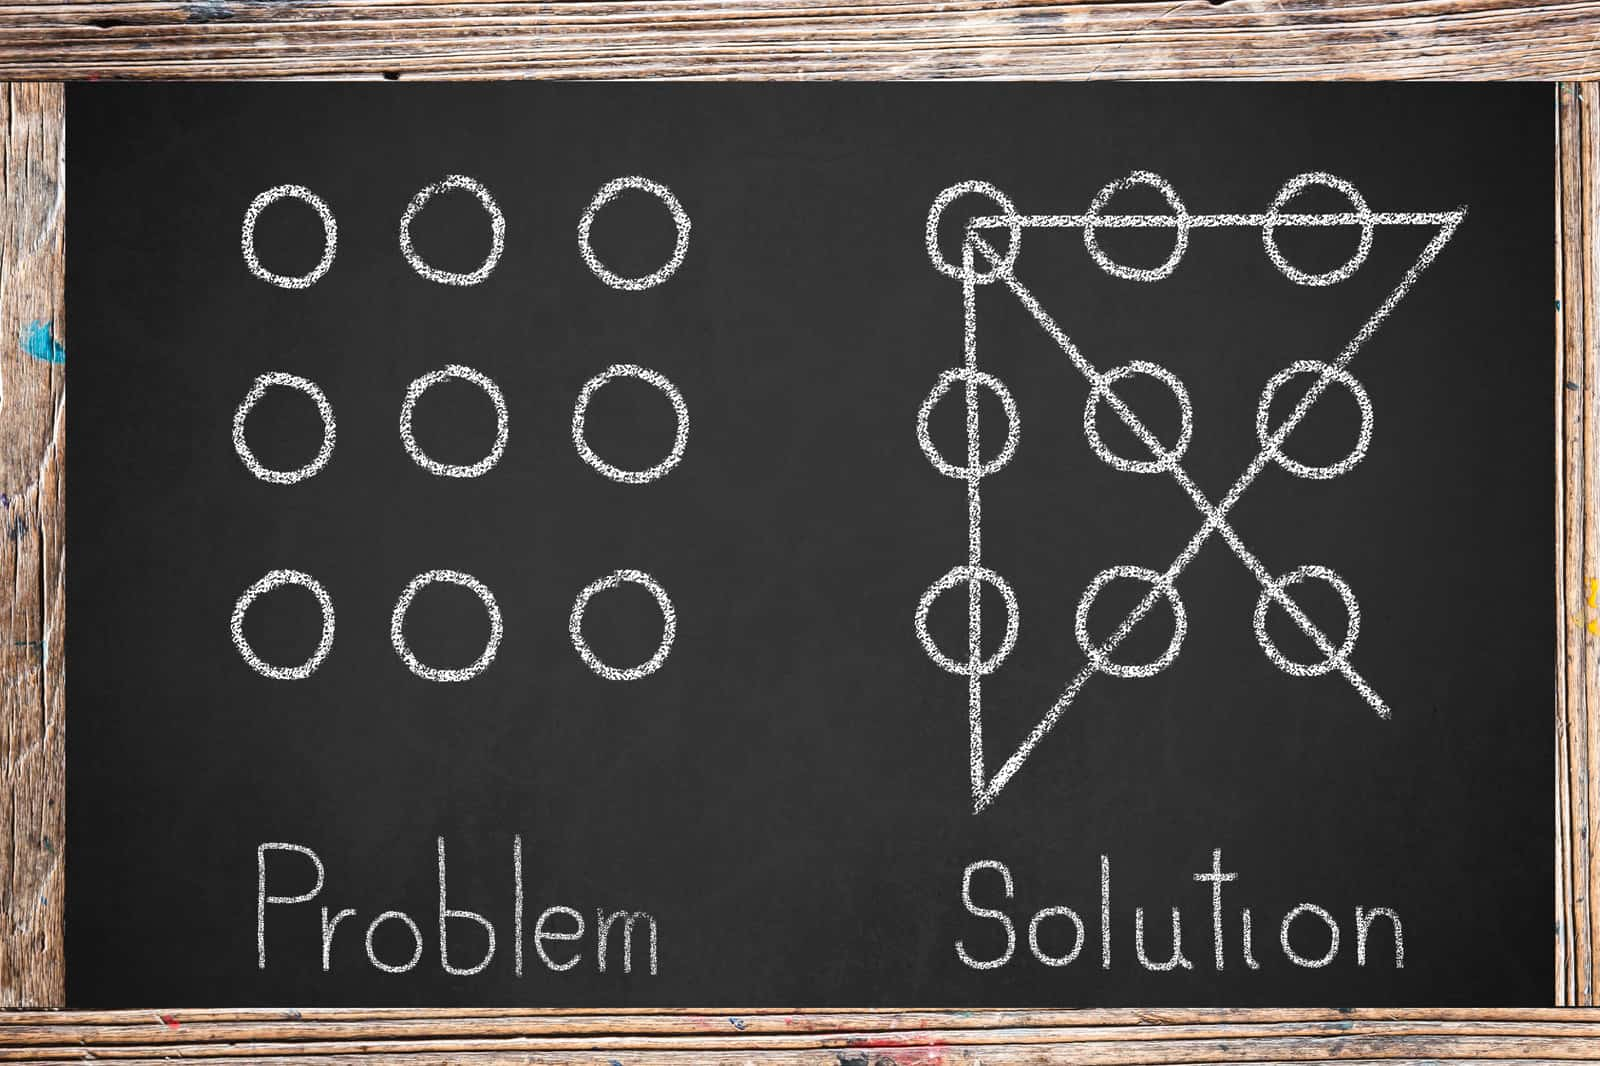
\includegraphics[width=0.5\textwidth]{ninedots}
\caption{Nine dot problem with solution.}
\label{fig:ninedots}
\end{figure}

\paragraph{What is spatial problem solving?}
In contrast to the more general approaches of problem solving described before, this work focuses on spatial problem solving and the question whether two people together perform better than a single person in a spatial problem solving task. 
Previous work in spatial problem solving has targeted fundamental processes of how individuals apply spatial learning, memory and planning. \cite{Waller2013} There exists also that investigate collaborative learning, but they do not focus on spatial problems. \cite{Dillenbourg1999} \cite{Hesse2015} Therefore the main goal of this work is to combine both spatial and collaborative problem solving.  

\paragraph{Why is spatial problem solving difficult to investigate?}
\paragraph{Why is virtual reality a good method to investigate spatial problem solving}
Since it is quite difficult to investigate and measure performance in collaborative spatial problem solving tasks in the real world a new task in virtual reality has been designed for this study. This task has been designed in a way that allows to investigate and compare problem solving performance both in individuals and in groups of two. The main benefit of using virtual reality to investigate spatial problem solving is the fact that the technical equipment allows to easily record data of how participants interact with the virtual environment (e.g. controller movements and rotations). Furthermore in a virtual environment the task, the position of participants and the environmental aspects of the scene can be easily manipulated and controlled. Therefore, virtual reality appears to be a very promising method to investigate collaborative spatial problem solving. 
\paragraph{Previous research in spatial Problem solving}
Only very few studies that compare to this approach can be found. One is the study by x + citation
- only investigate differences in interfaces solving a virtual reality task similar to the one here. It has been shown that head mounted displays are one of the best interfaces to investigate spatial problem solving. Since the technology has rapidly developed since the publication of this paper there are now much better interfaces and computer graphics available in order to create immersive virtual environments that allow interaction with different kinds of user input.
\paragraph{What is missing in previous research? Detailed performance measures and collaboration}
 The main goal of this study was to design a task in a virtual environment that is suitable to investigate and quantify the performance in problem solving both in individuals and groups of two people and also compare both variations. 

\paragraph{What is missing in previous research? Detailed performance measures and collaboration}

\section{Task Design}

In this section the design and idea behind the task which was used in the experiment will be explained. It is intended to focus on the task design only without considering the virtual reality aspects and and actual procedure which will be described in the methods sections. But is has to be kept in mind that the task is intended to be implemented in a 3D virtual environment which allows participants to almost freely interact and move. The challenge of designing a problem for a spatial problem solving experiment in a virtual 3D space is to find a balance between limiting the options and degrees of freedom participants have, but also allowing them enough possibilities to apply individual strategies within those limitations.


\paragraph{Requirement of the task}
When designing a task (or problem) for a problem solving experiment it is important to think about the complexity of the task. The literature differentiates between simple and complex tasks (problems). A simple task is characterized by having a clear initial  and goal state and all transitions and solution paths are known. Such tasks suit very well to investigate heuristics, search processes and systematic errors in problem solving. The main advantage is that simple tasks can be investigated well in experiments because they can be easily controlled. A complex task is mainly characterized by the fact that it is more closely related to real life problems, which makes them harder to be simulated in an experiment. It is important to understand that a simple task must not necessearily be easy to solve. The adjective "simple" refers only to the fact that the task's rules and its scope are limited to a few actions. The nine dot problem described before (Section \ref{sec:introduction} and Figure \ref{fig:ninedots}) can be categorized as a simple problem, because it is only possible to draw straight lines and it is not allowed to take the pen off the paper. Finding the solution still seems to be very difficult since only 10\% of the participants are able to solve the task. \cite{muesseler2015allgemeine} 
Since we want to be able to quantify and compare performances of individuals and groups of two, the main requirement for the task  was that is has to be a simple task. However, problem solving tasks in the 3D space are naturally pretty complex, because they allow all kinds of different movements and interactions. In the following the task components and rules will be described in detail in order to clarify its simple nature and also explain why this task is suitable to investigate and compare spatial problem solving for both individuals and groups of two.

\subsection{Task components and goal}
In this section the task components, the initial state and the goal state will be described.
The components of the task are 10 cubes and a solution space with 4 slots to hold one cube each. Every cube has a color on each of its 6 faces. The same color can be assigned at most to two faces of a cube. Since the colors vary in each trial a digit coding will be introduced in the following to describe the exact color configurations of all cubes. A color configuration of a cube consists of a mapping of all its faces to a digit code. Every digit code is a placeholder for a certain color. An example coding for one cube could look like this: 

front(f)=1, back(b)=0, left(l)=2, right(r)=0, top(t)=7, bottom(b)=8

The cube faces can have 9 different colors and therefore the digit coding has been defined that ranges from 0 to 8. The 9 different colors are required because the distractor cubes need to be colored with some distractor colors, which are not part of the goal state. Since the resulting cuboid has 6 faces there are six colors which are actually part of the goal state. The other 3 colors are the distractor colors. The complete digit coding for all 9 cubes can be found in Table \ref{tab:digit_coding}.

\begin{table}
\begin{center}
    \begin{tabular}{| l | | l | l | l | l | l | l |  l |}
    \hline
    Cube & front & back & left & right & top & bottom & type \\ \hline
    A & 1 & 0 & 2 & 0 & 7 & 8 & starting/solution \\ \hline
    B & 0 & 3 & 2 & 0 & 7 & 8 & solution \\ \hline
    C & 0 & 3 & 0 & 4 & 7 & 8 & solution \\ \hline
    D & 1 & 0 & 0 & 4 & 7 & 8 & solution \\ \hline
    E & 2 & 0 & 0 & 3 & 7 & 8 & distractor \\ \hline
    F & 0 & 3 & 0 & 5 & 7 & 8 & distractor \\ \hline
    G & 0 & 4 & 0 & 5 & 7 & 8 & distractor \\ \hline
    H & 0 & 3 & 0 & 6 & 7 & 8 & distractor \\ \hline
    I & 0 & 5 & 1 & 0 & 7 & 8 & distractor \\ \hline
    \end{tabular}
\end{center}
\caption{Digit coding of the color configuration for all cubes.}
\label{tab:digit_coding}
\end{table}

After taking a closer look at Table \ref{tab:digit_coding} one can see that 0, 7 and 8 are represented in each cube. This is because we made certain simplifications for the task in order to classify it as a simple problem. The digit 0 is always mapped to gray because we define gray as the faces 

\begin{table}
\begin{center}
    \begin{tabular}{| l | l |}
    \hline
    Digit code & color \\ \hline
    0 & gray \\ \hline
    1 & variable \\ \hline
    2 & variable \\ \hline
    3 & variable \\ \hline
    4 & variable \\ \hline
    5 & variable \\ \hline
    6 & variable \\ \hline
    7 & white \\ \hline
    8 & black \\ \hline
    \end{tabular}
\end{center}
\caption{Color mapping for digit codes. 0, 7 and 8 are always mapped to gray, black and white are because they do not change between trials. All other mappings are variable and allow to generate different instances of the same task that only differ in color. }
\label{tab:digit_coding}
\end{table}


The solution space consists of the 4 slots which have the same size as a cube and are arranged in a square from a top down view. In the initial state of the task the starting cube is already placed into the correct position in the solution space and the remaining 8 cubes are placed around the solution space. The remaining 8 cubes are rotated and positioned differently in each trial so that participants can not learn at which position the cubes for the solution are located (see Figure \ref{fig:vr_task_initialstate})

\begin{figure}[h]
\centering
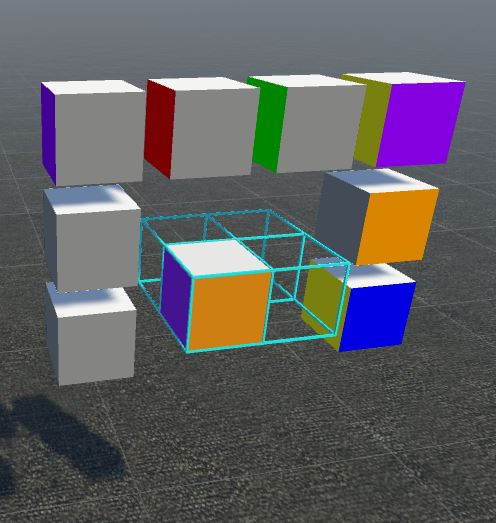
\includegraphics[width=0.75\textwidth]{vr_task_initialstate}
\caption{Initial state of the task: In the center - the solution space with the starting cube in light blue. Surrounding the solution space - the 9 remaining cubes to interact with. }
\label{fig:vr_task_initialstate}
\end{figure}

The goal state of the task is achieved when all slots of the solution space are filled with a cube and all 6 faces of the resulting cuboid are colored differently but also unicolored each. \ref{fig:vr_task_goalstate})

\begin{figure}[h]
\centering
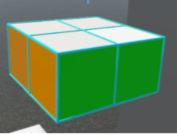
\includegraphics[width=0.5\textwidth]{vr_task_goalstate}
\caption{Goal state of the task: All slots of the solution space are filled with a cube and all 6 faces of the resulting cuboid are differently colored but also unicolored each. }
\label{fig:vr_task_goalstate}
\end{figure}

There are only 3 cubes that fit into a specific slot of the solution space in order to achieve the goal state. Those 3 cubes are the "goal cubes". The remaining 6 cubes are the "distractor cubes".

\subsection{Task rules and limitations}


\subsection{Task theory and tree structure}
Another requirement of the task is, that is must be possible to be solved in a reasonable amount of time 

restrctions? -> controlled

20 predifined tasks -> every participant does same task just in different order

The distractor cubes are colored in a way that they appear to fit into the goal state.

gray black white -> only rotate on vertical axis

Ideas behind the task design:	
- very controlled: reduce the variation of how participants could solve the task
- tree like solution path: 
--four potential ways to traverse the tree in order to get to the solution
--best case one traversion, worst case four traversions
--how many traversions participants need is random and not controlled, but it is possible to quantify how close participants were to one certain traversion path and the deviation from that can be defined as the error. (two times the same traversion = working memory error)

goal of task -> participants must optimize the way they apply the given strategy
\subsection{Implications for problem solving}

\section{Methods}

\subsection{Participants}
Twenty participants(10 female, 10 male; all right-handed) from the local university community participated in the experiment. Their age ranged from XX to XX years (M = XX, SD = XX). All participants were naive to the purpose of the experiment and had normal or corrected-to-normal vision. The experiment was approved by the ethics committee of the University of T\"ubingen, and was performed in accordance with the Declaration of Helsinki. Participants gave written informed consent prior to the experiment and were compensated with 8 Euro per hour for their participation. 

\subsection{Apparatus}
The virtual environment was displayed in stereo using an HTC Vive head-mounted-display (HMD) with a resolution of 1080 x 1200 pixels per eye (2160 x 1200 pixels combined). Inter-pupillary distance was measured with a pupilometer and set accoringly on the HTC Vive for each participant. Audio was recorded with a microphone plugged into the integrated audio input of the HTC Vive. Participants were standing during the whole experiment and viewed their virtual task in front of them.

Participants were run in an individual and a collaborative condition in which two participants worked together. Therefore the apparatus consisted of two HTC Vives of which each was connected to its own computer. The computers had the same hardware configuration (list PC specs?). In the individual condition participants were run in their own virtual environment solving a task alone (\ref{fig:individual_condition_setting}). In the collaborative condition two participants were run in a shared virtual environment solving the task together (\ref{fig:collaborative_condition_setting}). The synchronization between the two computers in the collaborative condition was done via UDP. Therefore the participants could collaborate in real time with very little to no delay or lag.

The virtual task consists of cubes and cube slots. The cubes can be picked up by moving the controller into a cube and pressing and holding the trigger button of the controller (there is both no collision between cubes and between cubes and the controller). When a cube is picked up it can be moved and rotated freely by the controller. When the cube is moved to the solution space it  automatically aligns ("snaps in") with the next closest cube slot.

%\begin{figure}
%\centering
%\includegraphics[width=0.8\textwidth]{individual_condition_setting.png}
%\caption{\label{fig:individual_condition_setting} XX.}
%\end{figure}

%\begin{figure}
%\centering
%\includegraphics[width=0.8\textwidth]{collaborative_condition_setting.png}
%\caption{\label{fig:collaborative_condition_setting} XX.}
%\end{figure}




\subsection{Procedure}
Participants were invited as a group of two people and did not know each other. In one group session the two participants solved the task on their own in a separate virtual environment and together in the same virtual environment. The sequence of single and collaborative was counter balanced among all groups. In both the single and collaborative condition participants solved 20 tasks of which all had the same design as described above and differed only in color. In the single condition participants viewed the task always from the same perspective, which means that the starting cube was always placed at the same position in the solution space.
In the collaborative condition we rotated the solution space after 10 trials, which means the starting cube is on one participant's side for the first 10 trials and on the other participant's side for the remaining 10 trials. 

The detailed procedure for the single condition will be explained in the following:
After having read the instructions of the task participants also received a verbal instruction by the experimenter. Before the actual 20 trials began participants had to solve two training trials in order to verify that the participant understood the task and the way it has to be solved. It was emphasized that it is important to always stick to the sequence of putting in and removing cubes as described above. Furthermore participants could experience that the starting cube can not be removed and is the only cube in the experiment with which the other cubes collide (that was important because we wanted to avoid that cubes can be places so that they overlap with the starting cube). Participants could also get used to the fact that the top color is always white and the bottom color is always black. The training trials could be started by the participant by holding a controller button for 2 seconds. When they start the training they saw the solution space surrounded by the 9 cubes which are all in reaching distance. They also saw the starting cube already being placed into the solution space. Above the task participants could see in which trial they currently are. In this case they would see "Training 1/2". Once they have finished a trial they can proceed with the next trial by pressing the controller button again for 2 seconds. 

Before the actual 20 trials start the experimenter repeats the most important instructions.Participants should try to solve the task as quickly and as accurately as possible. Also that they are not allowed to move around the problem space and should stay mostly stationary in their position with only a few steps to the sides allowed.
After the two training trials participants could start the actual trials as soon as they were ready by clicking a controller button again for 2 seconds. For the actual trial the experimenter would emphasize that participants should always make sure their solution is correct before proceeding with the next task. In case participants did not correctly solve a task and still proceed with the next task the experimenter took note in order to exclude the trial from the analysis.

The procedure for the collaborative solving of the task was mostly the same. The only difference was that just one participant was able to skip to the next trial and therefore the instructions were that participants had to agree on when to proceed with the next task.

%what needs to go in here is:

%instructions that were given to the participants
%training phase (how many trials...)
%counterbalance single / multi (counterbalanced - 10 each side)

\section{Results}
Data analysis was done by applying linear mixed models with the Kenward-Rodger degrees of freedom approximation. The random factors were the group number (= an individual number assigned to each group in the group condition), participant number (= an individual number assigned to each individual participant in the single condition) and the number of players(= either one or two). The only fixed factor was the number of players. 

 Although much more data has been recorded during the experiment this section will only cover the most relevant results that suit best to compare the performances of the single vs the group condition. 
 
 All data was automatically recorded from the time participants pressed the controller button to start the task to when they pressed the button again in order to skip to the next task. The data was based on the controller trajectories, rotations and user input  In the following the term "task duration" will be used to describe this duration in which data was recorded for an individual task.

\paragraph{Time to complete}
The time to complete is the average of all task durations.  Figure \ref{fig:results_duration} shows that the groups were much faster with an average of 50 seconds compared to single participants with an average of 80 seconds. The output of the linear mixed model was F:(1,18.99) = 52.049, p < 0.001 

\begin{figure}[h]
\centering
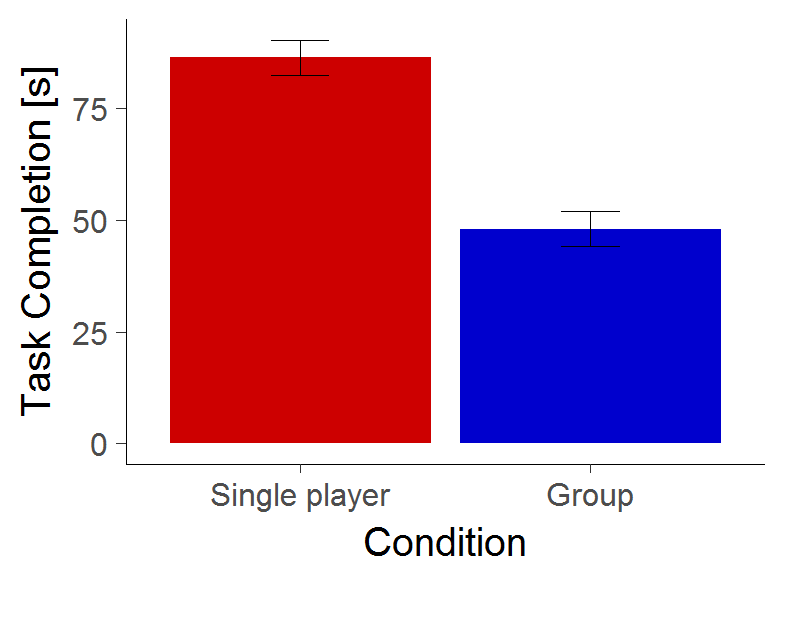
\includegraphics[width=0.5\textwidth]{results_duration}
\caption{Average time in seconds to complete the task in singel and group condition.} \label{fig:results_duration}
\end{figure}

\paragraph{Rotation sum of cubes}
The rotation sum of cubes is the sum of rotations made by one participant during the task duration. In the group condition we summed up the rotations of both group members first and calculated the averages over the group sums. Figure \ref{fig:results_rotations} shows that the average rotation sum for groups with an average of 5000 degrees was significantly less compared to single participants with an average of 8000 degrees. For the rotation sum a the smaller value indicates the better performance because the less a participant rotates a cube the more confident and efficient the participant is expected to be at solving the task. The output of the linear mixed model was F:(1,18.99) = 12.164, p < 0.01.

\begin{figure}[h]
\centering
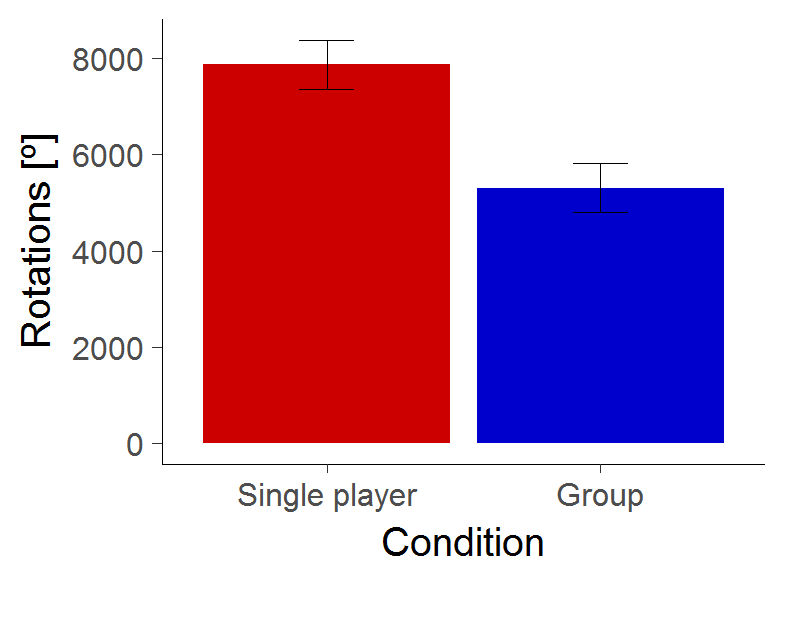
\includegraphics[width=0.5\textwidth]{results_rotations}
\caption{Sum of rotations in degrees.}
\label{fig:results_rotations}
\end{figure}

\paragraph{Number of cube snap-outs}
The number of cube snap-outs it the number of how many times a participant took a cube back out from the problem space during the task duration. Figure \ref{fig:results_snap_outs} shows that groups needed much less snap-outs with an average of 2.1 snap-outs compared to single participants with an average of 4.5 snap-outs. 
Snap-outs can be categorized in two classes: "necessary" and "unnecessary" snap-outs. Necessary snap-outs are the ones which are part of the task design which means participants are supposed to try certain solution paths and if a path was not successful they need to snap-out some cubes and snap-in new ones until they successfully finish the task. It is possible though that participants try the same or similar solution path more than one time and therefore have to do unnecessary snap-outs. For the number of cube snap-outs a smaller value indicates the better performance, because it means that less unnecessary snap-out were made. The average of necessary snap-outs is expected to be equally distributed with an expectancy value of 2.0. In other words scoring an average of 2.0 snap-outs is an indicator of almost perfect performance to which the group condition is very close with 2.1.
The output of the linear mixed model was F:(1,18.99)=22.112, p < 0.001.

\begin{figure}[h]
\centering
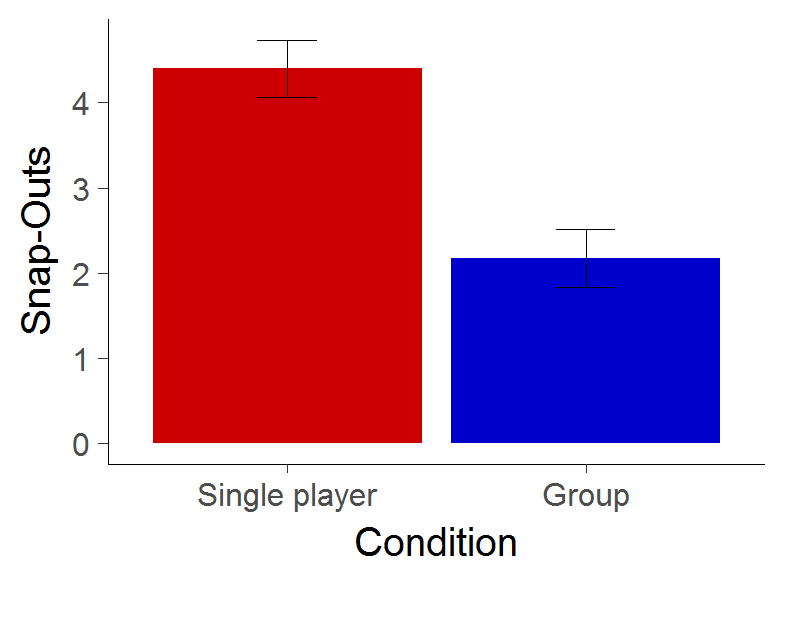
\includegraphics[width=0.5\textwidth]{results_snap_outs}
\caption{Example of a parametric }
\label{fig:results_snap_outs}
\end{figure}

\paragraph{Number of solution paths}

The output of the linear mixed model was F:(1,18.99)=4.565, p < 0.05.


\begin{figure}[h]
\centering
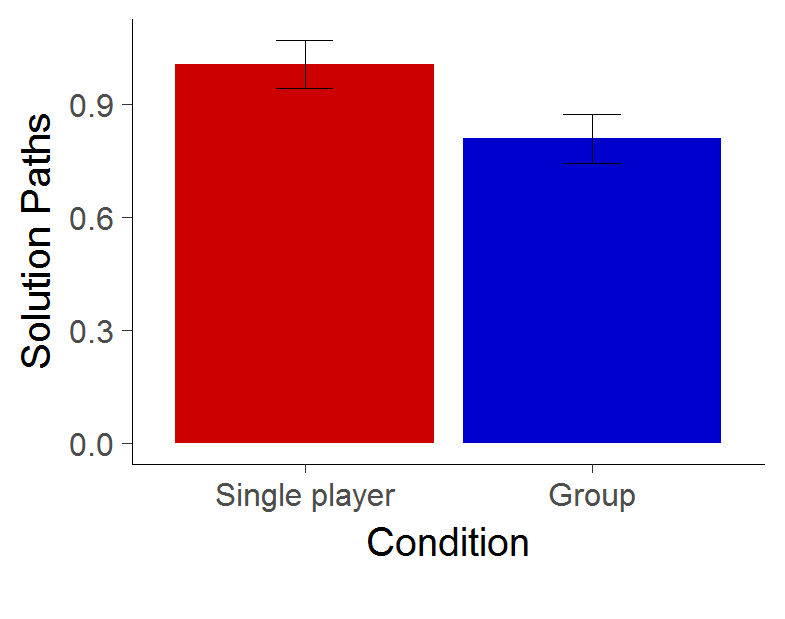
\includegraphics[width=0.5\textwidth]{results_solution_paths}
\caption{Example of a parametric }
\end{figure}

\paragraph{Error}

The output of the linear mixed model was F:(1,18.99)=9.338, p < 0.01.


\begin{figure}[h]
\centering
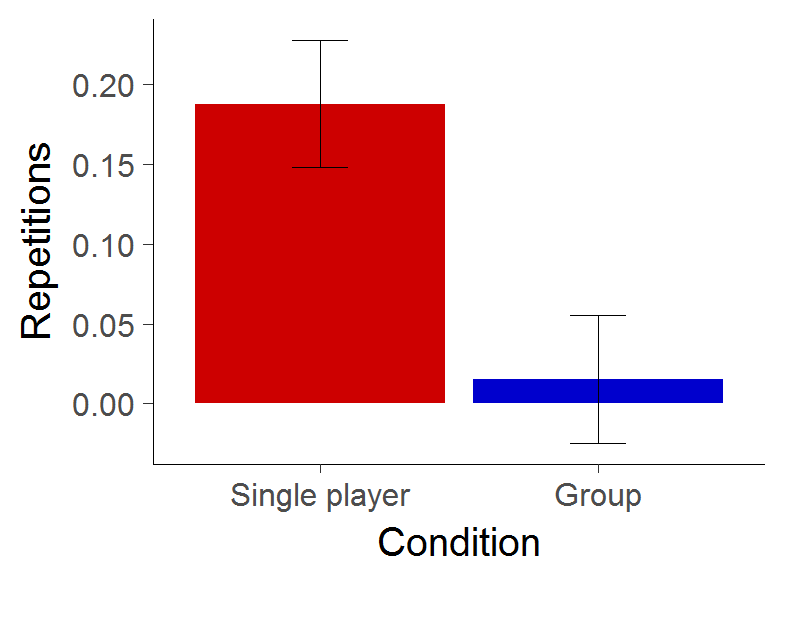
\includegraphics[width=0.5\textwidth]{results_un_error}
\caption{Example of a parametric }
\end{figure}


\section{Discussion}
- 
- design of the task, which can be used in follow up experiments -> explain variations
- explain main results -> 2 vs 1 -> costs of working memory vs shared representation and planning


\bibliographystyle{plainnat}
\bibliography{references}

\end{document}
